\chapter{Heat Modeling of Integrated Devices}
\label{ch:heatmodeling}
\section{Heat Models using physical device models}
\subsection{Other Methods}
\subsubsection{RC-\,Networks}
\section{Extension to On-Line Evolution of Heat Models}

\section{Temperature Measurement Methods}

\subsection{Built-In Temperature Sensors}
PTAT = proportional to absolute temperature


\begin{math}
	V_{PTAT} = 10 \times \frac{kT}{q}\times ln(p)
\end{math}

\begin{itemize}
	\item Boltzman's constant $k = 1.38 \times 10^{-23}$
	\item Temperature in Kelvin $T$
	\item Charge on an electron $q = 1.6 \times 10^{-19}C$
	\item Emission current density ratio $p = 10$
\end{itemize}

$V_{PTAT}$ is digitized by the ADC (10 bit output).

\begin{math}
	T[\symbol{23}^{\circ}C] = \frac{ADCcode\times 503.957}{1024} - 273.15
\end{math}

\cite{Xilinx2011a, Bakker1996}

	+- 4�C internal temp sensor \cite{Xilinx2011a}
	
	VCC and temperature proportionally ! \cite{Ruthing2012}

\subsection{Ring Oscillators}

Nowadays, a widely spread technique to measure the internal on-chip temperatures of \ac{FPGA}-based systems are based on \acp{RO}. These devices are composed of an odd number of inverters, which are connected in a chain. The endmost inverter's output is fed back to the first inverter. Figure~\ref{pic:simple_ro} depicts such a basic \ac{RO}. This leads to a device without a stable condition, causing each inverter's output to oscillate, i.\,e. the output $Q$ toggles between $0$ and $1$ and maximum speed with frequency $f_{osc}$. A longer inverter chain leads to a lower frequency and in addition to less power consumption \cite{Velusamy2005}.
It is because of the fact that the \ac{RO}'s frequency $f_{osc}$ is inversely proportinal to the on-chip temperature \cite{Lopez-Buedo2002}, that \acp{RO} can be used to measure the temperature on any location on the \ac{FPGA}. The output frequency $f_{osc}$ is dependant on the curcuit's delay. Furthermore, it is also known that \acp{RO} can be used in order to measure delay, leakage and dynamic power \cite{Zick2012}. 

\begin{figure}[h]
		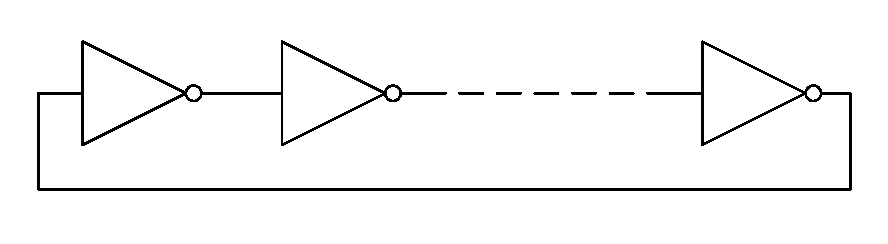
\includegraphics[width=\textwidth]{__pics/RO.pdf}
		\caption{A basic Ring Oscillator, consisting of an odd number of inverters}
		\label{pic:simple_ro}	
	\end{figure} 

\subsubsection{Methodology}

Measuring the internal on-chip temperature necessarily requires knowledge about the frequency $f_{osc}$ of the \ac{RO}. In order to estimate the frequency, several approaches \cite{Sayed2011, Lopez-Buedo2002, Velusamy2005, Happe} make use of \acp{RO} combined with a capture counter, which will be clocked with the oscillating output signal $Q$. Put simply, the capture counter samples the number $S$ of oscillations in $Q$, which allows the computation of $f_{osc}$. The realization of this behavior is depicted in Figure~\ref{pic:Temp_Sensor} \cite{Ruthing2012}.

\begin{figure}[h]
		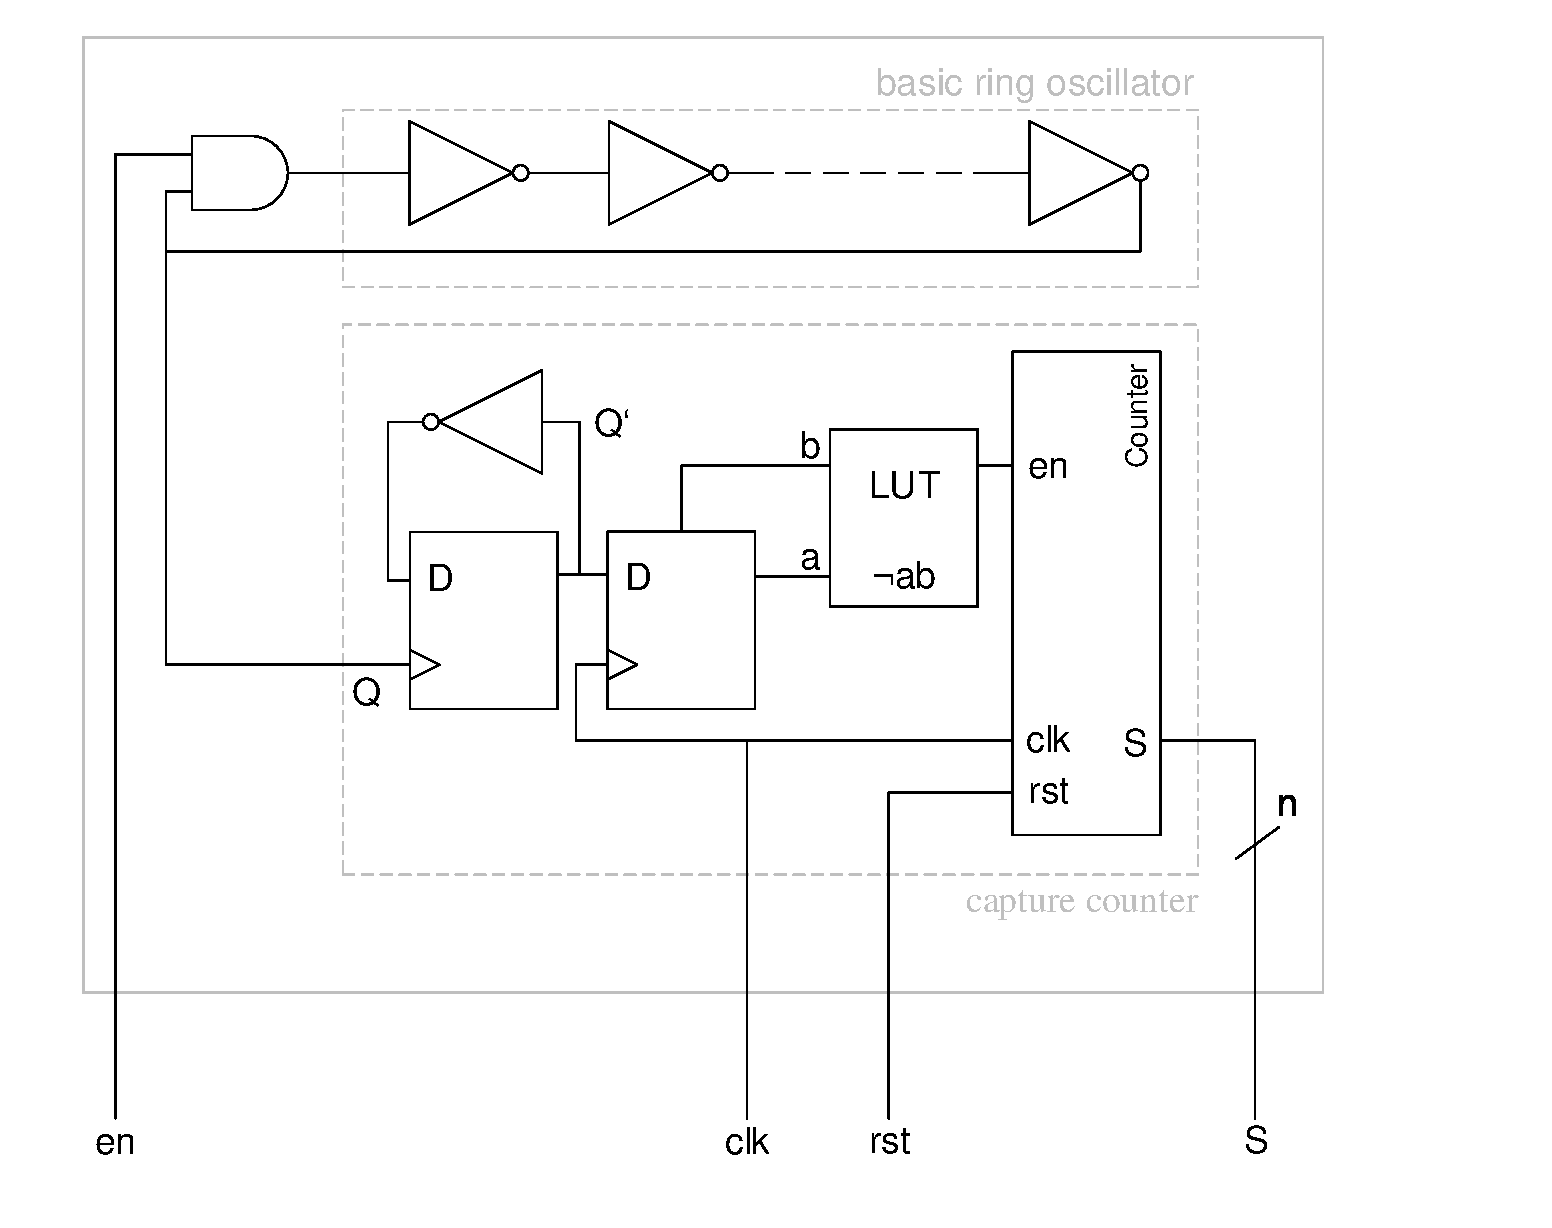
\includegraphics[width=1.15\textwidth]{__pics/Temp_Sensor.pdf}
		\caption{Simplified schematic of a temperature sensor with capture counter cf. \cite{Ruthing2012}}
		\label{pic:Temp_Sensor}	
	\end{figure} 
	
However, there are also differences in implementing the \ac{RO}-based temperature sensor. These variable parameters are: number of inverters, system routing, length of measurement period $t_m$ and the possible use of latches between the inverters. 
The use of latches was proposed in order to minimize the impact of routing \cite{Zick2012}. For \acp{FPGA} designs, it is advisable to use latches instead of the additional wiring between the inverters. 

The benefits of designing on an \ac{FPGA} are the reconfigurability. This possible due to the \acp{CLB} of which the \ac{FPGA} is composed. The \ac{CLB} however comprises slices, which contain \acp{LUT} and \acp{FF}. 
Hence, by using \acp{LUT} for the \ac{RO}'s inverters, the \acp{FF} can be used as latches without significant additional wiring.

In contrast to previous approaches, which used seven \cite{Happe} or eleven inverters \cite{Lopez-Buedo2002, Velusamy2005} and no latches, a high-performance \ac{RO}-based temperature sensor comprises 23 inverters and 24 latches \cite{Ruthing2012}. The quality of the \ac{RO} is derived by sensor resolution and sensor noise/deviation.
In addition to the utilization, the optimal measurement period $t_m$ should not exceed the maximum length of $2^{16}$ clock cycles, which is $655\,\mu s$, when the counter samples with 100\,MHz. For longer measurement periods, there is a risk of self-heating, since \acp{RO} may lead to considerable temperature gradients \cite{Agne2013}.

As previously pointed out, the optimal measurement with the proposed temperature sensor includes the following steps \cite{Ruthing2012}:

\begin{itemize}
	\item Enable \ac{RO} with 23 inverters and 24 latches
  \item Wait $2^{12}$ -- $2^{16}$ clock cycles so that the \ac{RO} can gain a constant frequency
  \item Sample $Q'$ for $t_m$ clock cycles
  \item Disable the \ac{RO}
  \item Read out the counter value $S$.
\end{itemize}

\subsubsection{Calibration Methods}

Given the sensor count $S$ of \ac{RO}-based temperature sensors, it is not possible to predict a function that maps $S$ to a temperature $T$. Instead, the sensors need to be calibrated with an precalibrated device, such as the built-in thermal diode. 
While the device is heated up and cooled down afterwards, the sensor counts $S$ and the temperature provided by the built-in thermal diode $T_{diode}$ is read in regular time intervals. For each sensor the linear mapping function is then determined by partial regression \cite{Lopez-Buedo2002, Ruthing2012}. Section~\ref{sec:tempgen} will give an overview of most common and useful methods for heating up the \ac{FPGA}.

\subsection{Infrared Cameras}

Besides the above-named on-chip solutions of measuring the internal temperature, there is also the possibility to use \ac{IR} cameras. 

For instance, \cite{Ebi2011} measured a spatial thermal gradient of 2\symbol{23}$^{\circ}C$ over 10mm on a Xilinx Virtex II \ac{FPGA} using an infrared camera.

direct vision to silicon and can not be employed in actual working conditions \cite{Lopez-Buedo2004}


\cite{Nowroz2011, Ebi2011, Agne2013}
expensive, cannot be deployed in field, scientific use, evaluation or calibration

\begin{figure}[h]
		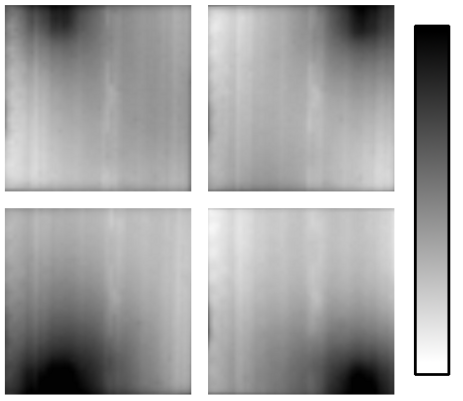
\includegraphics[width=\textwidth]{__pics/infra_heater}
		\caption{Four infrared images of the \ac{FPGA} with temperatures from 80\symbol{23}$^{\circ}C$ (white) to 95\symbol{23}$^{\circ}C$ (black) cf. \cite{Agne2013}}
		\label{pic:heater_infrared}	
	\end{figure} 


\subsection{Discussion on Accuracy}

\section{Temperature Generation Methods}
\label{sec:tempgen}